\chapter{TP-Link devices : the programmable WiFi Access Points}
 %TODO donatien
 \section{Goal of the TP-Link device}
  The aim of the TP-Link is to collect RSSI from connected wifi devices allowing the server to compute the actual position of the android device. To achieve that we created two programs, one which catches packets that are transiting through the network, then retrieves the RSSI to finally store its values. The other program creates a socket and waits for the server to connect. When connected, it sends an average value of all RSSI concerning one mobile device (identified with its MAC addres) to the server.
  \section{Sequence diagram of the communication}
   
     \begin{figure}[H]
      \centering
       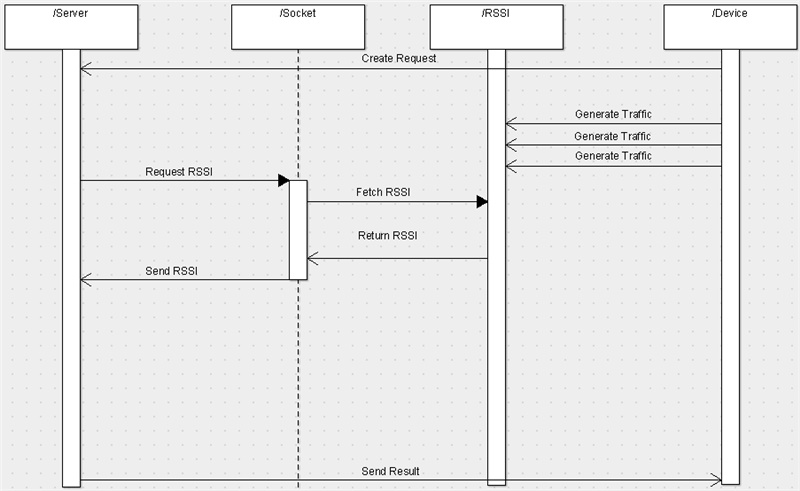
\includegraphics[scale = 0.5]{img/tp_link/tplink_sq_diag}
      \caption{Sequence Diagram representing the communication between a TP-Link device and the server.}
      \label{fig:tplink_seq_diagram}
     \end{figure}
    ~\\
\indent The Socket and RSSI processes are running on the AP OS, the server and the mobile device are based on other environments. The device connects to the server for a specific request and then generates traffic which is caught by the AP. It then fills its RSSI list. Later on, the server asks the Socket process the average of the measured RSSIs, the socket accesses the RSSI list and returns the request value.

  \section{Algorithms}
   \subsection{Rssi retrievement}
    Retrieving the RSSI for a packet is realized using the pcap library. Firstly we need to create the packet listener using the function \textit{pcap\textunderscore open\textunderscore live} which takes the interface we want to listen to. Then we enter a loop where we catch a packet using \textit{pcap\textunderscore next}, we check if the packet is correct by checking the first two bits of the header frame control. Then we compute the offset of the RSSI in bytes by looking at the radio tap flags in the \textit{it\textunderscore present} array. \\
\indent Once we have the RSSI, which is filtered if unreliable (value of 4dbm for example), and the MAC address we insert it to the RSSI list. So first we lock the semaphore to insure concurrent access with regard to the socket thread, and then we add the value for the right MAC address. We also clear all outdated values (which occurrs when one is in the list for more than one second). Finally the semaphore is unlocked.

   \subsection{Socket connections}
    To communicate the RSSIs to the server, a socket is opened on a separate thread listening to the port 3000. In order to do so, the standard socket library is used. First we create the socket using the \textit{socket} function. Then one applies some setup to make the socket listen to the port 3000 and finally one loops where connections are accepted, handled and closed.\\
\indent When a connection is accepted the handler first waits for a new string to arrive. It is then translated into a MAC address. A semaphore is then locked to insure concurrent access with the RSSI thread and the RSSI average value is computed for all RSSIs for one device. The lock is then released and a string is sent back through the socket according to this format : "MAC;RSSI". Finally the socket is closed and one loops again.

  \section{Encountered Problems}
  The main problem encountered when handling the TP-Link devices was, for an unknown reason, that the RSSI in the packet was not correctly positioned (at the good index inside the caught packet's header). So for certain configurations of the TP-LINK, RSSI measurement was impossible. However, for other TP-Link devices, everything worked out. We are still trying to find a solution for this bug.